\documentclass[12pt, twoside]{article}
% \documentclass[12pt, twoside]{article}
\usepackage[letterpaper, margin=1in, headsep=0.2in]{geometry}
\setlength{\headheight}{0.6in}
%\usepackage[english]{babel}
\usepackage[utf8]{inputenc}
\usepackage{microtype}
\usepackage{amsmath}
\usepackage{amssymb}
%\usepackage{amsfonts}
\usepackage[nomessages]{fp} %\FPeval{\var-name}{2*sin(pi/6)}
\usepackage{siunitx} %units in math. eg 20\milli\meter
\usepackage{yhmath} % for arcs, overparenth command
\usepackage{tikz} %graphics
\usetikzlibrary{quotes, angles, arrows, arrows.meta}
\usepackage{graphicx} %consider setting \graphicspath{{images/}}
\usepackage{parskip} %no paragraph indent
\usepackage{enumitem}
\usepackage{multicol}
\usepackage{venndiagram}

\usepackage{fancyhdr}
\pagestyle{fancy}
\fancyhf{}
\renewcommand{\headrulewidth}{0pt} % disable the underline of the header
\raggedbottom
\hfuzz=2mm %suppresses overfull box warnings

\usepackage{hyperref}
\usepackage{float}

\title{IB}
\author{Chris Huson}
\date{October 2025}

\fancyhead[LE]{\thepage}
\fancyhead[RO]{\thepage \\ First \& last name: \hspace{2.25cm} \,\\ Grade: \hspace{2.25cm} \,}
%\fancyhead[RO]{First \& last name: \hspace{2.25cm} \,\\ \,}
\fancyhead[LO]{La Scuola d'Italia / Huson / IB Math: Sequences \\* 22 October 2025}

\begin{document}

\subsubsection*{1.11 Homework: Series; due Monday 27 October}
\begin{enumerate}[itemsep=0.5cm]

\item Given a geometric sequence with $u_1=3$ and $r=2.25$
  \begin{enumerate}
      \item Find $u_5$.
      \item Find $S_5$, the sum of the first five terms of the sequence.
      \item $S_k=7980$. Find $k$ algebraically.
  \end{enumerate}

\item In an arithmetic sequence, the first term is 3 and the second term is 7.
    \begin{enumerate}
        \item Find the common difference. \hfill [2 marks]
        \item Find the tenth term. \hfill [2 marks]
        \item Find the sum of the first ten terms of the sequence. \hfill [2 marks]
    \end{enumerate}

\item The first three terms of an arithmetic sequence are $u_1 = 0.3, u_2 = 1.5, u_3 = 2.7$.
    \begin{enumerate}
        \item Find the common difference. \hfill [2 marks]
        \item Find the 30th term of the sequence. \hfill [2 marks]
        \item Find the sum of the first 30 terms. \hfill [2 marks]
    \end{enumerate}

\item The first three terms of a geometric sequence are $u_1 = 0.64, u_2 = 1.6, u_3 = 4$.
    \begin{enumerate}
        \item Find the value of $r$. \hfill [2 marks]
        \item Find the value of $S_6$. \hfill [2 marks]
        \item Find the least value of $n$ such that $S_n > 75,000$. \hfill [3 marks]
    \end{enumerate}

\item Consider a geometric sequence where the first term is 768 and the second term is 576.\\
Find the least value of $n$ such that the $n$th term of the sequence is less than 7. \hfill [6 mks]

\item Consider the following sequence of figures.
    \begin{figure}[H]
        \centering
        \includegraphics[width=0.6\textwidth]{../graphics/sequence-boxes.png}
    \end{figure}
    \begin{enumerate}
        \item Figure 1 contains 5 line segments.\\
        Given that Figure $n$ contains 801 line segments, show that $n=200$. \hfill [3 marks]
        \item Find the total number of line segments in the first 200 figures. \hfill [3 marks]
    \end{enumerate}

\newpage
\subsubsection*{Sequences and series with logarithms}

\item The first three terms of a geometric sequence are $\ln x^{16}, \ln x^{8},\ln x^{4}$, for $x>0$.
    \begin{enumerate}
        \item Find the common ratio. \hfill [3 marks]
        \item Solve $\displaystyle \sum_{k=1}^{\infty} 2^{5-k} \ln x = 64$. \hfill [5 marks]
    \end{enumerate}

\item An arithmetic sequence has the first term $\ln a$ and a common difference $\ln 3$.\par
The 13th term in the sequence is $8 \ln 9$. Find the value of $a$. \hfill [6 marks]

\item The first two terms of an infinite geometric sequence, in order, are \par 
$2 \log_2 x$, $\log_2 x$ where $x > 0$.
    \begin{enumerate}[itemsep=0.5cm]
        \item Find $r$. \hfill [2 marks]
        \item Show that the sum of the infinite sequence is $4 \log_2 x$. \hfill [2 marks]
        \item The first three terms of an arithmetic sequence, in order, are $\log_2 x$, $\log_2 (\frac{x}{2})$, $\log_2 (\frac{x}{4})$, where $x>0$.\\
        Find $d$, giving your answer as an integer. \hfill [4 marks]
        \item Let $S_{12}$ be the sum of the first 12 terms of the arithmetic sequence.\\
        Show that $S_{12} = 12 \log_2 x -66$. \hfill [2 marks]
        \item Given that $S_{12}$ is equal to half the sum of the infinite geometric sequence, find $x$, giving your answer in the form $2^p$, where $p \in \mathbb{Q}$. \hfill [3 marks]
    \end{enumerate}

       
\end{enumerate}
\end{document}

\newpage
\subsubsection*{Graphing}

\item Graph $y=400(.85)^{2x}-6$ on the set of axes below.
\begin{center}
    \begin{tikzpicture}
    \draw[step=0.25in,gray,very thin] (0,0) grid (12.7,12.7);
    \draw[thick,->] (0,0) -- (13,0); node[anchor=north west] {x};
    \draw[thick,->] (0,0) -- (0,13); node[anchor=south east] {y};
    \foreach \x in {1.27} \draw (\x cm,3pt) -- (\x cm,-3pt) node[anchor=north] {$1$};
    \foreach \x in {12.7} \draw (\x cm,3pt) -- (\x cm,-3pt) node[anchor=north] {10};
    \foreach \y in {3.2} \draw (3pt,\y cm) -- (-3pt,\y cm) node[anchor=east] {100};
    \foreach \y in {12.7} \draw (3pt,\y cm) -- (-3pt,\y cm) node[anchor=east] {400};
    \end{tikzpicture}
\end{center} %Alg2 Regents Jun2017

\item The expression $(x + a)(x + b)$ can not be written as
\begin{enumerate}
    \item $a(x + b)+ x(x + b)$
    \item $x^2 + (a + b)x + ab$
    \item  $x^2 + abx + ab$
    \item $x(x + a)+ b(x + a)$
\end{enumerate}

